\documentclass[12pt]{extarticle}

\usepackage[a4paper,left=3cm,right=3cm,top=2cm,bottom=2.5cm]{geometry}
\usepackage{graphicx}
\usepackage{titlesec}
\usepackage{authblk}
\usepackage[utf8]{inputenc}
\usepackage[T1]{fontenc}
\usepackage[ngerman]{babel}
\usepackage{setspace}
\usepackage{unicode-math}
\usepackage{fontspec}
\usepackage{tabularx}
\usepackage{multirow}
\usepackage{hyperref}

\setmainfont{TeX Gyre Pagella}
\setsansfont{TeX Gyre Heros}
\setmonofont{TeX Gyre Cursor}

\graphicspath{{../supplements/img/}, {../supplements/}, {../raumpläne/}}

\renewcommand\Authand{ und }
\renewcommand\Authands{ und }

\newcommand{\labinfo}[3]{
    \begin{tabularx}{\textwidth}{lX}
        \textbf{Art der Nutzung} & #1 \\
        \textbf{Arbeitsplätze} & #2 \\
        \textbf{Verantwortlich} & #3 \\
    \end{tabularx}

    \vspace{3mm}
}

\title{
    \bfseries
    \sffamily
    Hygienekonzept für die Labore des Lehrstuhls für Medieninformatik
}

%\author{Christian Wolff \\ \href{mailto:christian.wolff@ur.de}{christian.wolff@ur.de}}
\author{Christian Wolff}
\author{Andreas Schmid}
\author{Alexander Bazo}
\author{Martin Kocur}
\author{Raphael Wimmer}
\author{Martin Brockelmann}
\author{Patricia Böhm}
\author{Victoria Böhm}
\author{Thomas Schmidt}

\affil{Lehrstuhl für Medieninformatik, Universität Regensburg}

\begin{document}

\onehalfspacing
\maketitle

\noindent
Um die Labore des Lehrstuhls für Medieninformatik zu benutzen, sind die in diesem Dokument aufgeführten Hygieneregeln einzuhalten.
Werden die Labore für Nutzerstudien verwendet, so gelten zusätzliche Vorsichtsmaßnahmen.
Die Hygieneregeln wurden passend zur COVID-19-Situation am 15. Mai 2020 aufgestellt.
Sie werden regelmäßig überprüft und an die aktuelle Situation angepasst.

\section{Allgemeine Informationen zu diesem Dokument}

Zu den Laboren des Lehrstuhls für Medieninformatik zählen:

\begin{itemize}
    \item Das Future Interaction Lab
    \begin{itemize}
        \item Usability-Labor (PT 3.0.27)
        \item Werkstatt (PT 3.0.28)
        \item Besprechungsraum (PT 3.0.28A)
    \end{itemize}
    \item Der Eyetracking-Classroom (SG 5.20/21)
    \item Versuchsraum 4 in der TechBase
    \begin{itemize}
        \item VR4 Labor
        \item VR4 Studio
        \item VR4 Werkstatt
    \end{itemize}
\end{itemize}

\noindent
Dieses Dokument enthält

\begin{itemize}
    \item Allgemeine Rahmenbedingungen und Hygieneregeln zur Nutzung der Labore
    \item Maßnahmen des Lehrstuhls, um die Umsetzung der Hygienemaßnahmen in den Laboren zu gewährleisten
    \item Spezifische Hinweise zum Benutzen von Head-Mounted Displays (HMD)
    \item Zusätzliche Regeln für die Durchführung von Nutzerstudien
    \item Individuelle Regelungen für jedes der Labore
\end{itemize}

\noindent
Zusätzlich hängen diesem Dokument an

\begin{itemize}
    \item Raumpläne der einzelnen Labore
    \item Hinweisschilder zu den Hygienemaßnahmen
\end{itemize}


\section{Allgemein Rahmenbedingungen für die Labornutzung}

\noindent
Für alle Labore des Lehrstuhls für Medieninformatik gilt:

\begin{enumerate}
    \item Grundsätzlich ist die Labornutzung nur gestattet, wenn
    \begin{enumerate}
        \item Die Laborinfrastruktur für die Tätigkeit unverzichtbar ist.
        \item Ein zeitliches Verschieben der Tätigkeit nicht möglich ist.
        \item Alle Hygienevorschriften eingehalten werden.
    \end{enumerate}
    \item{Jede Labornutzung muss vorher bei den zuständigen Mitarbeitenden des Lehrstuhls für Medieninformatik mit einer ausreichenden Begründung beantragt werden.
    Diese entscheiden einmal pro Woche für jeden Fall individuell anhand eines Kriterienkatalogs, ob die Nutzung des Labors gestattet wird und vergibt Laborzeiten dann die Nutzer*Innen.}
    \item{Vor der Erstnutzung eines Labors durch eine Person ist eine persönliche Einweisung in die Arbeits- und Hygienerichtlinien durch die zuständigen Mitarbeitenden des Lehrstuhls für Medieninformatik notwendig.}
    \item{Personen mit bestätigter Sars-CoV-2-Infektion oder typischen Krankheitssymptomen ist der Zutritt zu allen Räumen des Lehrstuhls für Medieninformatik untersagt.
    Vor jeder Nutzung eines der Labore muss die eigene Symptomatik mit einer Checkliste abgeglichen werden.}
    \item{Beginn und Ende jeder Labornutzung sind über ein digitales Formular zu dokumentieren.
    Dabei sind Nutzungszeitraum, Name, Handynummer und E-Mail-Adresse anzugeben.
    Dies gilt auch für Proband*Innen von Nutzerstudien.
    Am Ende jeder Benutzung müssen verwendete Gegenstände und Tischoberflächen desinfiziert werden.
    Die wird in einem Hygieneprotokoll festgehalten.}
    \item{Angemessene Handhygiene, ein Mindestabstand von 1,5 Metern, sowie die Hust- und Niesetikette, sind einzuhalten.
    Ist mehr als eine Person im Raum, ist zusätzlich ein Mund- und Nasenschutz zu tragen.
    Darauf wird in jedem Labor mit Schildern hingewiesen.}
    \item{Labore mit Fenster sind spätestens alle 45 Minuten für mindestens 5 Minuten zu lüften.}
\end{enumerate}


\section{Maßnahmen zur praktischen Umsetzung der Regeln}

\begin{enumerate}
    \item Die Laborräume werden nur an Einzelpersonen vergeben, Arbeit in Projektgruppen ist nicht gestattet.
    \item Wenn möglich werden Räume für längere zeitliche Blöcke am Stück vergeben, sodass möglichst wenig personeller Wechsel in den Laboren stattfindet.
    \item Hardware und Werkzeug werden wenn möglich personalisiert vergeben, sodass sie während eines Zeitraums nur von einer Person verwendet werden.
    \item In allen Laborräumen werden Händedesinfektionsmittelspender, Sprühflaschen mit Flächendesinfektionsmittel und Einwegmasken bereitgestellt.
    \item Arbeitsbereiche in den Laboren werden so eingerichtet, dass ein Mindestabstand von 1,5 Metern besteht. Zusätzliche Tische und Stühle werden wenn möglich entfernt, sodass die Räume eine geringe Affordanz bieten, gegen den Mindestabstand und die maximale Personenzahl zu verstoßen.
    \item In jedem Labor werden folgende Hinweisschilder angebracht:
    \begin{enumerate}
        \item Handhygiene
        \item Hust- und Niesetikette
        \item Abstandsregeln
        \item Maskenpflicht
        \item Kurzfassung Hygieneregeln
        \item Symptome COVID-19
    \end{enumerate}
    \item Das Einhalten der Regeln wird vom Laborpersonal regelmäßig kontrolliert.
    \item Wir behalten uns vor, Verstöße gegen die Hygieneregeln mit Ausschluss aus dem Laborbetrieb zu ahnden.
\end{enumerate}


\section{\sout{Arbeit mit Head-Mounted Displays (HMD)}}\label{sec:hmd}

\noindent
\emph{\textbf{Änderung 23.11.2021:} Abschnitt wegen Redundanz gestrichen}
\medskip

\medskip
\noindent
\sout{Anwendungen im Bereich der Virtual und Augmented Reality sind Teil vieler Arbeiten in der Medieninformatik.
Bei der Entwicklung von Anwendungen für HMDs wird durch personalisierte Geräte gewährleistet, dass ein HMD nur von ein und derselben Person verwendet wird.
Nach der Verwendung von HMDs, beispielsweise für die Entwicklung von Anwendungen oder für Proband:innen bei Nutzerstudien, werden diese desinfiziert.}

\medskip
\noindent
\sout{Bei der Durchführung von Nutzerstudien, bei denen Proband:innen ein HMD tragen, ist dem in Kapitel \ref{subsec:nutzerstudien_hmd} beschriebenen Ablauf zu folgen.}


\section{Durchführung von Nutzerstudien}\label{sec:nutzerstudien}

\noindent
In der Medieninformatik werden neue Interaktionstechniken und User Interfaces entwickelt und evaluiert, sowie bestehende untersucht und verbessert.
Ein etabliertes Vorgehen ist dabei das Durchführen von Nutzerstudien, bei denen Proband*innen in einer kontrollierten Laborumgebung mit diesen Systemen interagieren.
Einige Studien werden auch in der virtuellen Realität durchgeführt und setzen spezielle Hardware wie Head-Mounted Displays oder Tracking-Anzüge für ein Motion-Capturing-System voraus.

\medskip
\noindent
Das Durchführen von Nutzerstudien im Labor ist nur dann gestattet, wenn die Laborinfrastruktur unbedingt benötigt wird und die Studie nicht remote durchgeführt werden kann.
Vorerst sind Interviews, Fokusgruppen und ähnliche Studien beispielsweise per Videochat durchzuführen.

\noindent
Beim Durchführen von Nutzerstudien sind folgende Maßnahmen zu beachten:

\begin{enumerate}
    \item Name, E-Mail-Adresse und Handynummer aller Proband*innen, sowie der Zeitraum der Studie werden dokumentiert um mögliche Infektionsketten nachvollziehen zu können. Diese Daten werden nach 30 Tagen gelöscht.
    \item Nach jeder ProbandIn werden alle Kontaktgegenstände und -flächen desinfiziert und, wenn möglich, der Laborraum für mindestens fünf Minuten gelüftet.
    \item Auch für Proband*innen gilt: Befindet sich mehr als eine Person im Raum, muss ein Mund- und Nasenschutz getragen werden.
    \item Es wird jederzeit ein Mindestabstand von 1,5 Metern zu Probanden eingehalten.
    \item Nur ein/e ProbandIn befindet sich gleichzeitig im Labor. Wenn möglich sollen Proband*innen vor der Studie außerhalb des Gebäudes warten. Um Warteschlangen zu vermeiden, soll ausreichend viel Zeit zwischen einzelnen Proband*innen eingeplant werden.
\end{enumerate}

\noindent
Nutzerstudien, die das Tragen von Hardware am Körper voraussetzen, weisen ein erhöhtes Risiko der Schmierinfektion auf.
Deshalb wird vorerst die Anzahl an ausgeschriebenen Abschluss- und Projektarbeiten, bei denen diese Art von Studien durchgeführt werden, reduziert und wenn möglich nach alternativen Themen, Projektideen und Durchführungsmethoden gesucht.
Für Arbeiten, für die keine alternativen Methoden existieren und für die das Benutzen von am Körper getragener Hardware erforderlich ist, dürfen Nutzerstudien lediglich unter erhöhten Sicherheitsmaßnahmen durchgeführt werden.

\subsection{Durchführung von Studien mit Head-Mounted Displays}\label{subsec:nutzerstudien_hmd}

Da durch die Verwendung von Head-Mounted Displays (HMD) ein höheres Infektionsrisiko besteht, ist bei Nutzerstudien mit derartigen Geräten ein genaues Ablaufprotokoll einzuhalten.

\subsubsection*{Vorbereiten und Anbringen des HMD}

{
\singlespacing
\begin{itemize}
    \item Sauberes HMD (nach 72-stündiger Quarantäne) aus verschließbarer Box herausholen
    \item HMD mit einem “Einmalüberzug” (wird nach einmaliger Benutzung entsorgt) vorbereiten
    \item ProbandIn auf markierten Platz verweisen 
    \item VersuchsleiterIn trägt Handschuhe
    \item VersuchsleiterIn tritt ausschließlich seitlich an ProbandIn heran
    \item VersuchsleiterIn hält HMD von unten am Gehäuse und bittet ProbandIn sich nach vorne mit Gesicht auf die Brille zu beugen 
    \item VersuchsleiterIn befestigt Kopfgurt 
    \item Controller liegt vor ProbandIn bereit 
    \item VersuchsleiterIn zieht Handschuhe aus und entsorgt diese in verschließbaren Mülleimer
    \item VersuchsleiterIn desinfiziert sich die Hände
    \item VersuchsleiterIn setzt sich an den Kontrollrechner in mindestens 1,5 Meter Abstand zu ProbandIn
\end{itemize}
}

\subsubsection*{Abnehmen des HMD}

{
\singlespacing
\begin{itemize}
    \item VersuchsleiterIn trägt frische Handschuhe
    \item VersuchsleiterIn tritt seitlich an Proband*in
    \item VersuchsleiterIn lockert Kopfgurt
    \item ProbandIn zieht dann Brille nach vorne weg
    \item HMD Brillensheet und Handschuhe in verschließbaren Mülleimer entsorgen
    \item HMD für 72 Stunden in Quarantäne setzen
    \begin{itemize}
        \item Verschließbare Box öffnen und HMD hineinlegen
        \item Box mit Datum und Uhrzeit versehen
    \end{itemize}
    \item VersuchsleiterIn und ProbandIn desinfizieren sich die Hände
\end{itemize}
}

\subsection{Durchführung von Studien mit Tracking-Anzügen}\label{subsec:nutzerstudien_mocap}

Wird bei einer Studie das Motion-Capturing-System verwendet, so müssen Proband*innen Ganzkörperanzüge mit speziellen Markern tragen.
Durch den direkten Körperkontakt besteht ein erhöhtes Infektionsrisiko, weshalb ein genaues Ablaufprotokoll zum An- und Ablegen des Anzugs, sowie dessen Reinigung und Aufbewahrung, einzuhalten ist.

\subsubsection*{Zu Beginn der Studie}

{
\singlespacing
\begin{itemize}
    \item VersuchsleiterIn trägt Handschuhe
    \item Anzug für ProbandIn vorbereiten und zur Verfügung stellen
    \item ProbandIn auf markierten Platz verweisen 
    \item VersuchsleiterIn beschreibt Schritt für Schritt wie man den Motion Capture Anzug anzieht
\end{itemize}
}

\subsubsection*{Nach der Studie}

{
\singlespacing
\begin{itemize}
    \item Motion Capture Anzüge in Quarantäne setzen
    \item verschließbare Box für Anzüge öffnen und Anzug hineinlegen
    \item Anzug in Box zur Reinigung bringen
\end{itemize}
}


\section{Individuelle Richtlinien für jedes der Labore}\label{sec:labore}
\emph{\textbf{Änderung: 02.09.2021:} Informationen zur RLT-Anlage im VR4 hinzugefügt.}
\noindent
\emph{\textbf{Änderung: 02.07.2021:} Quarantänezeit für HMDs entfernt.}

Der Lehrstuhl für Medieninformatik verfügt über drei Labore: Das \emph{Future Interaction Lab} (FIL) im Gebäude PT3, den Eyetracking-Classroom im Sammelgebäude (SG) und Versuchsraum 4 (VR4) in der TechBase.

\medskip
\begin{figure}[h]
    \sffamily
    \centering
    \frame{
    \begin{tabular}{ m{1.1cm} m{3cm} }
        \multicolumn{2}{l}{\textbf{Legende}} \\
        \vspace{2mm}
        
\includegraphics[width=1cm]{arbeitsplatz} & Arbeitsplatz \\
        
\includegraphics[width=1cm]{tisch} & Tisch \\
        
\includegraphics[width=1cm]{durchgang} & Tür \\
        
\includegraphics[width=1cm]{fenster} & Fenster \\
        
\includegraphics[width=1cm]{trennwand} & Trennwand \\
    \end{tabular}
    \quad
    \begin{tabular}{ m{1.1cm} m{5cm} }
        \vspace{2mm}
        \includegraphics[width=1cm]{flächendesinfektion} & Flächendesinfektionsmittel \\
        
\includegraphics[width=1cm]{handdesinfektion} & Händedesinfektionsmittel \\
        
\includegraphics[width=1cm]{waschbecken} & Waschbecken \\
        
\includegraphics[width=1cm]{hinweisschilder} & Hinweisschilder \\
    \end{tabular}
    }
\end{figure}

\noindent
Das FIL ist mit Trennwänden ausgestattet, die bei Bedarf geöffnet werden können, ist aber normalerweise in drei einzelne Räume mit eigenen Eingangstüren aufgeteilt.
Alle Räume sind an eine Lüftungsanlage angeschlossen, die die Raumluft nach außen umwälzt und Frischluft von außen ansaugt.
Das Usability-Labor und die Werkstatt verfügen über keine weiteren Lüftungsmöglichkeiten.
Im Besprechungsraum befindet sich ein Fenster, über das zusätzlich gelüftet werden kann.
Alle Räume verfügen über einen separaten Zugang zum Gang. 

\medskip
\begin{figure}[h]
    \label{fig:raumplan_fil}
    \centering
    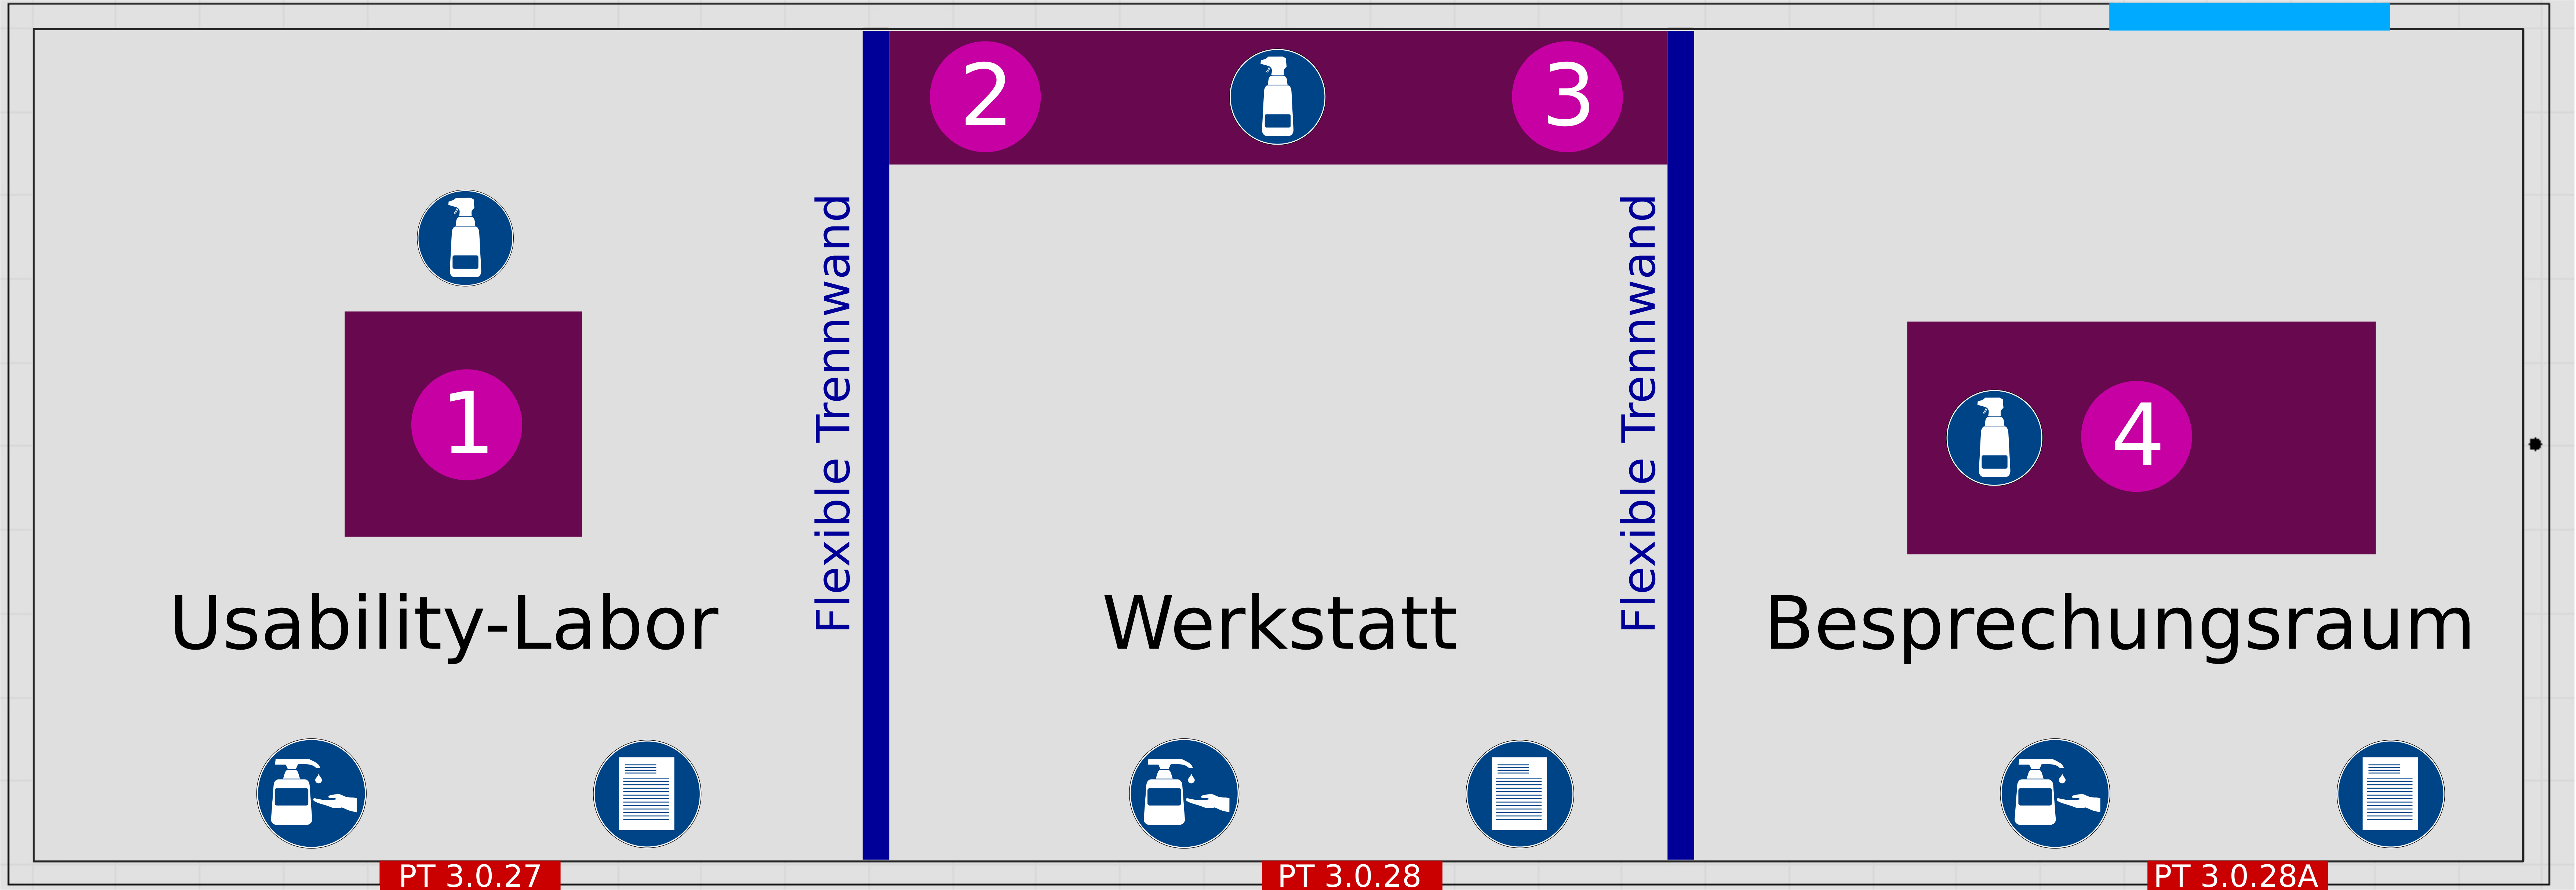
\includegraphics[width=0.9\textwidth]{fil_konzept}
    \caption{Raumplan Future Interaction Lab}
\end{figure}

\noindent
VR4 ist in drei Bereiche aufgeteilt, jedoch muss der Hauptraum (VR4 Labor) durchquert werden, um in die anderen beiden Bereiche (VR4 Studio und VR4 Werkstatt) zu gelangen. Da sich VR4 nicht im Universitätsgebäude sondern in der TechBase befindet, wurde zusätzlich mit deren Hausverwaltung geklärt, dass auch Studierende und Proband:innen das Gebäude betreten dürfen.
VR4 verfügt über eine raumlufttechnische Anlage, welche über Außenluft betrieben wird und über geeignete Filter verfügt.
Zu- und Abluft sind voneinander getrennt und sämtliche Filter werden in regelmäßigem Turnus vom Facility Management der TechBase gewechselt.

\medskip
\begin{figure}[h]
    \label{fig:raumplan_vr4}
    \centering
    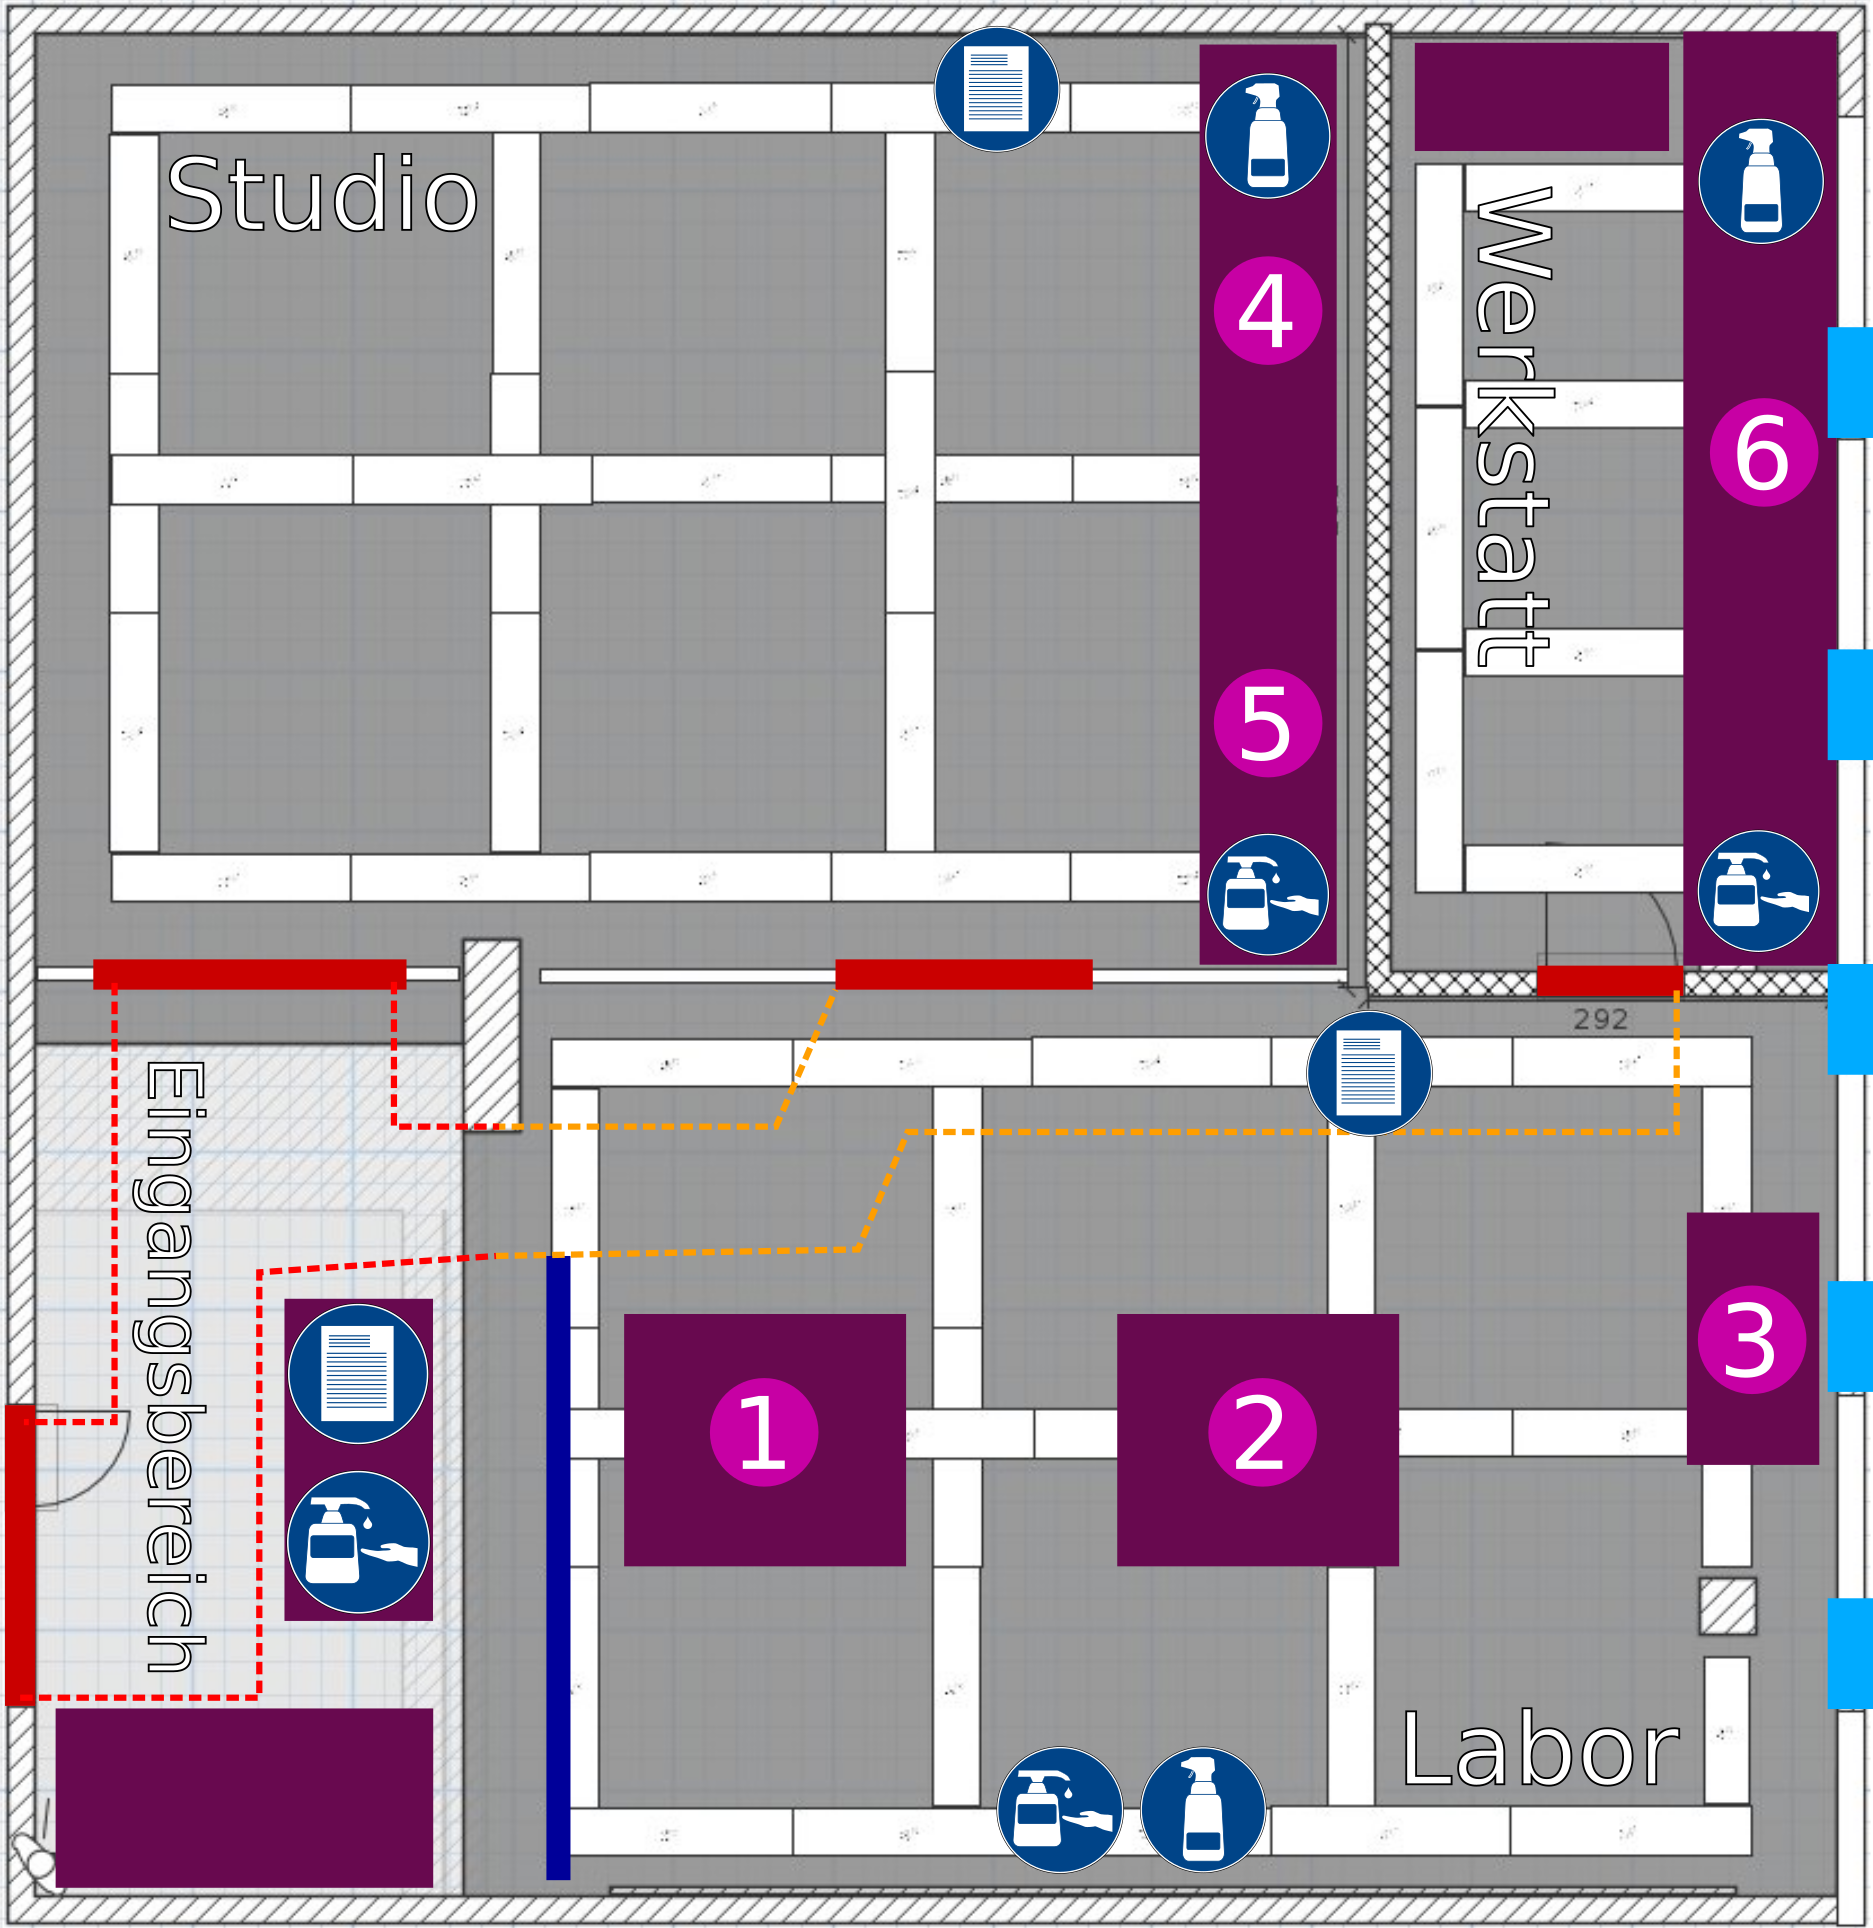
\includegraphics[width=0.65\textwidth]{vr4_konzept}
    \caption{Raumplan TechBase VR4}
\end{figure}

Im Eingangsbereich des VR4 wird mit Schildern auf die aktuell geltenden Auflagen hingewiesen.
Dort steht auch Händedesinfektionsmittel bereit.
Der normalerweise offene Durchgang vom Eingangsbereich zum Hauptraum des Labors wird mit Bühnenmolton abgehängt.
So kommen Personen, die im Hauptraum arbeiten nicht mit denen in Kontakt, die nur ins Studio müssen - insbesondere Proband:innen von Nutzerstudien.
Im Hauptraum werden zwei feste Arbeitsplätze an interaktiven Tischen, sowie ein Eyetracker, eingerichtet. Sie werden so platziert, dass ein Mindestabstand von 1,5 Metern stets eingehalten wird.
Diese Arbeitsplätze sind personalisiert und werden dauerhaft nur von einer Person benutzt.

Im Studio befinden sich zwei Bildschirmarbeitsplätze mit ausreichendem Sicherheitsabstand für die Entwicklung von Virtual-Reality-Anwendungen.
Wenn im Studio Nutzerstudien durchgeführt werden, betreten und verlassen Proband:innen den Raum nur über die Tür zum Eingangsbereich.
Desinfektionsmittel und Hinweise zum Anlegen und Abnehmen von Head-Mounted Displays und Tracking-Anzügen stehen bereit.
Die Werkstatt wird über einen gekennzeichneten Weg durch den Hauptraum betreten.
Sie bietet einen Arbeitsplatz und die Tür darf nur zum Betreten und Verlassen des Raums geöffnet werden.

Hauptraum und Werkstatt können über Fenster an der Ostseite gelüftet werden.
Das Studio verfügt über keine eigenen Fenster, deshalb kann nur über den Hauptraum gelüftet werden, sofern dieser nicht belegt ist.
Aus diesem Grund muss das Studio bei jedem Besetzungswechsel für mindestens drei Stunden leer stehen, sodass sich eventuell in der Luft befindliche Keime absetzen können.

\medskip
\noindent
Der Eye-Tracking-Classroom besteht aus einem Laborbereich, einem ehemaligen CIP-Pool, sowie einem Server-, Beobachtungs- und Entwicklungsbereich. Beide Räume verfügen über separate Zugänge über den Gang und sind durch eine Zwischentür miteinander verbunden.
Die Belüftung erfolgt über die Fenster, die in jedem der Räume vorhanden sind.

\medskip
\begin{figure}[h]
    \label{fig:raumplan_eyetracking}
    \centering
    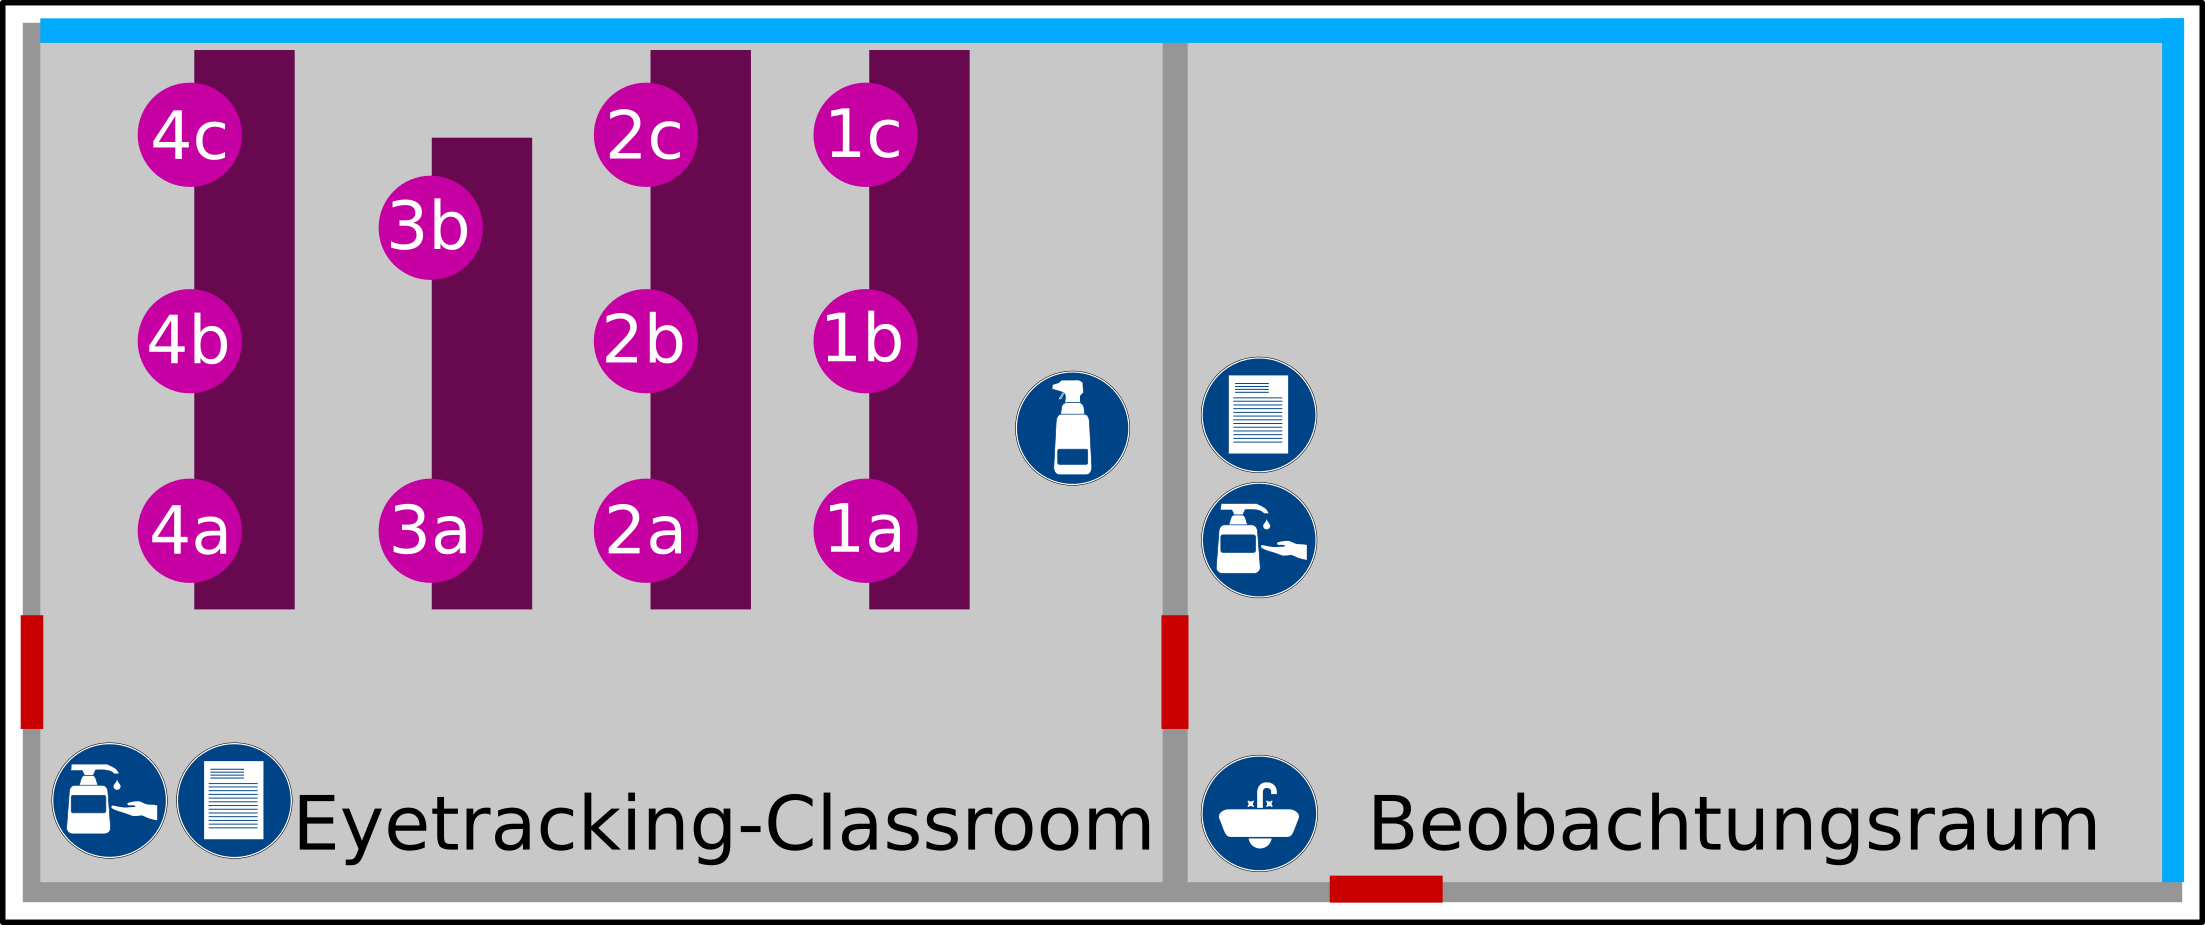
\includegraphics[width=0.7\textwidth]{eyetracking-classroom_konzept}
    \caption{Raumplan Eyetracking-Classroom}
\end{figure}

\medskip
\noindent
Im Folgenden werden die Art der Nutzung während der Einschränkungen, sowie die praktische Umsetzung der Hygienemaßnahmen für jeden der Räume dargestellt.

\subsection{Future Interaction Lab: Usability-Labor}\label{subsec:labore_fil_labor}

\labinfo{Klassische Benutzerstudie, Entwicklungsarbeiten, Medienproduktion}{1}{Alexander Bazo, Christoph Härtl}

\noindent
Das Usability-Labor dient vorrangig der Durchführung von Nutzerstudien, insbesondere solcher Experimente, die eine ``Alltagssituation'' als Testumgebung erfordern. Dazu sind neben einem PC-Arbeitsplatz auch ein Sofa und Fernseher vorhanden.
Der Arbeitsplatz kann zusätzlich auch für Entwicklungsarbeiten und die Medienproduktion eingesetzt werden.
Bei Verwendung der vorhandenen Geräte (Workstations) muss nach Gebrauch eine Desinfektion der Eingabegeräte (Maus \& Tastatur) erfolgen.

\medskip
\noindent
Bei Verwendung des Raums für die Durchführung von Nutzerstudien wird die Fläche  durch Öffnen der Trennwand zu der angrenzenden Werkstatt erweitert. Damit ist dann auch eine Trennung von Ein- und Ausgängen für die Testpersonen möglich.
Die räumlichen und einrichtungstechnischen  Beschränkungen im Labor schließen Studien mit mehr als einem Probanden aus.
Insgesamt sollten im Raum nicht mehr als zwei Personen (Proband:in und Testleiter:in) anwesend sein. Denkbar sind zusätzliche Beobachter:in in einem der angrenzenden Räume. Entsprechende Videotechnik steht im Labor zur Verfügung.

\subsection{Future Interaction Lab: Werkstatt}\label{subsec:labore_fil_werkstatt}

\labinfo{Entwicklungsarbeiten, Medienproduktion}{2}{Alexander Bazo, Christoph Härtl}

\noindent
Die Werkstatt im Future Interaction Lab dient vorrangig der (Software-) Entwicklungsarbeit.
Zusätzlich befindet sich hier eine ca.
2,5 x 2,5m große Freifläche, die für Tests- und Studien von VR-Arbeiten verwendet werden kann.
Die Arbeitsplätze sind an einer der Längsseiten angebracht. Unter Berücksichtigung der notwendigen Abstandsregeln können hier bis zu zwei Personen gleichzeitig arbeiten.
Die Arbeitsflächen wurden weitestgehend freigeräumt, um eine einfache Reinigung und Desinfektion zu erlauben.
Nutzer:innen werden angehalten, diesen Zustand beizubehalten.
Bei Verwendung der vorhandenen Geräte (Workstations) muss nach Gebrauch eine Desinfektion der Eingabegeräte (Maus \& Tastatur) erfolgen.
Hier kann zusätzliche Hardware für den regelmäßigen Austausch der angeschlossenen Geräte verwendet werden.
Grundsätzlich kann auch eine Nutzung der Workstations nur bei Verwendung eigener Eingabegeräte gestattet werden.

\medskip
\noindent
Bei Verwendung des Raums für die Durchführung von Nutzerstudien wird die Fläche durch Öffnen der Trennwand zu einem der angrenzenden Räume (Besprechungsraum oder Usability-Raum) erweitert.
Damit ist dann auch eine Trennung von Ein- und Ausgängen für die Testpersonen möglich.

\subsection{Future Interaction Lab: Besprechungsraum}\label{subsec:labore_fil_besprechungsraum}

\labinfo{Vorübergehend ausgesetzt}{-}{Alexander Bazo, Christoph Härtl}

\noindent
Im Besprechungsraum des FIL befinden sich ein Konferenztisch, sowie ein Smartboard.
Außerdem ist er der einzige Teilbereich des FIL mit einem Fenster.
Im Normalbetrieb des Labors wurde der Raum neben Besprechungen hauptsächlich für Nutzerbefragungen und Fokusgruppen genutzt.
Da diese Nutzung eine erhöhte Infektionsgefahr birgt und leicht durch digitale Lösungen (etwa per Videokonferenz) ersetzt werden kann, wird der Raum bis auf Weiteres nicht dafür verwendet.
Stattdessen wird die flexible Trennwand zur FIL Werkstatt dauerhaft geöffnet, sodass diese über das Fenster im Besprechungsraum gelüftet werden kann.
Besprechungen mit bis zu vier Teilnehmer:innen sind unter Beachtung der Abstandsregeln grundsätzlich möglich.
Im Anschluss ist die Desinfektion der Tischoberfläche, der Tastatur / Maus / Fernbedinung Beamer und der Türklinken erforderlich.

\subsection{PT 3.0.30}\label{subsec:labore_pt3.0.30}

\labinfo{VR-Studien}{1}{Martin Kocur}

\noindent
Der Raum  PT 3.0.30 wird vorübergehend als zusätzliches Labor genutzt, um Nutzerstudien im Bereich Virtual Reality (VR) durchzuführen.
Dadurch soll für eine Entlastung der anderen Labore des Lehrstuhls gesorgt werden.
Es dürfen sich maximal zwei Personen (Versuchsleiter/in und Proband/in) gleichzeitig im Raum befinden.
Eine Desinfektion nach jeder Nutzung der verfügbaren und genutzten Hardware (HMDs, Tastaturen, Mäuse, Arbeitsflächen) sowie das Lüften des Raumes nach dem Wechsel von Proband:innen ist zwingend erforderlich.

\medskip
\begin{figure}[h]
    \label{fig:raumplan_pt3.0.30}
    \centering
    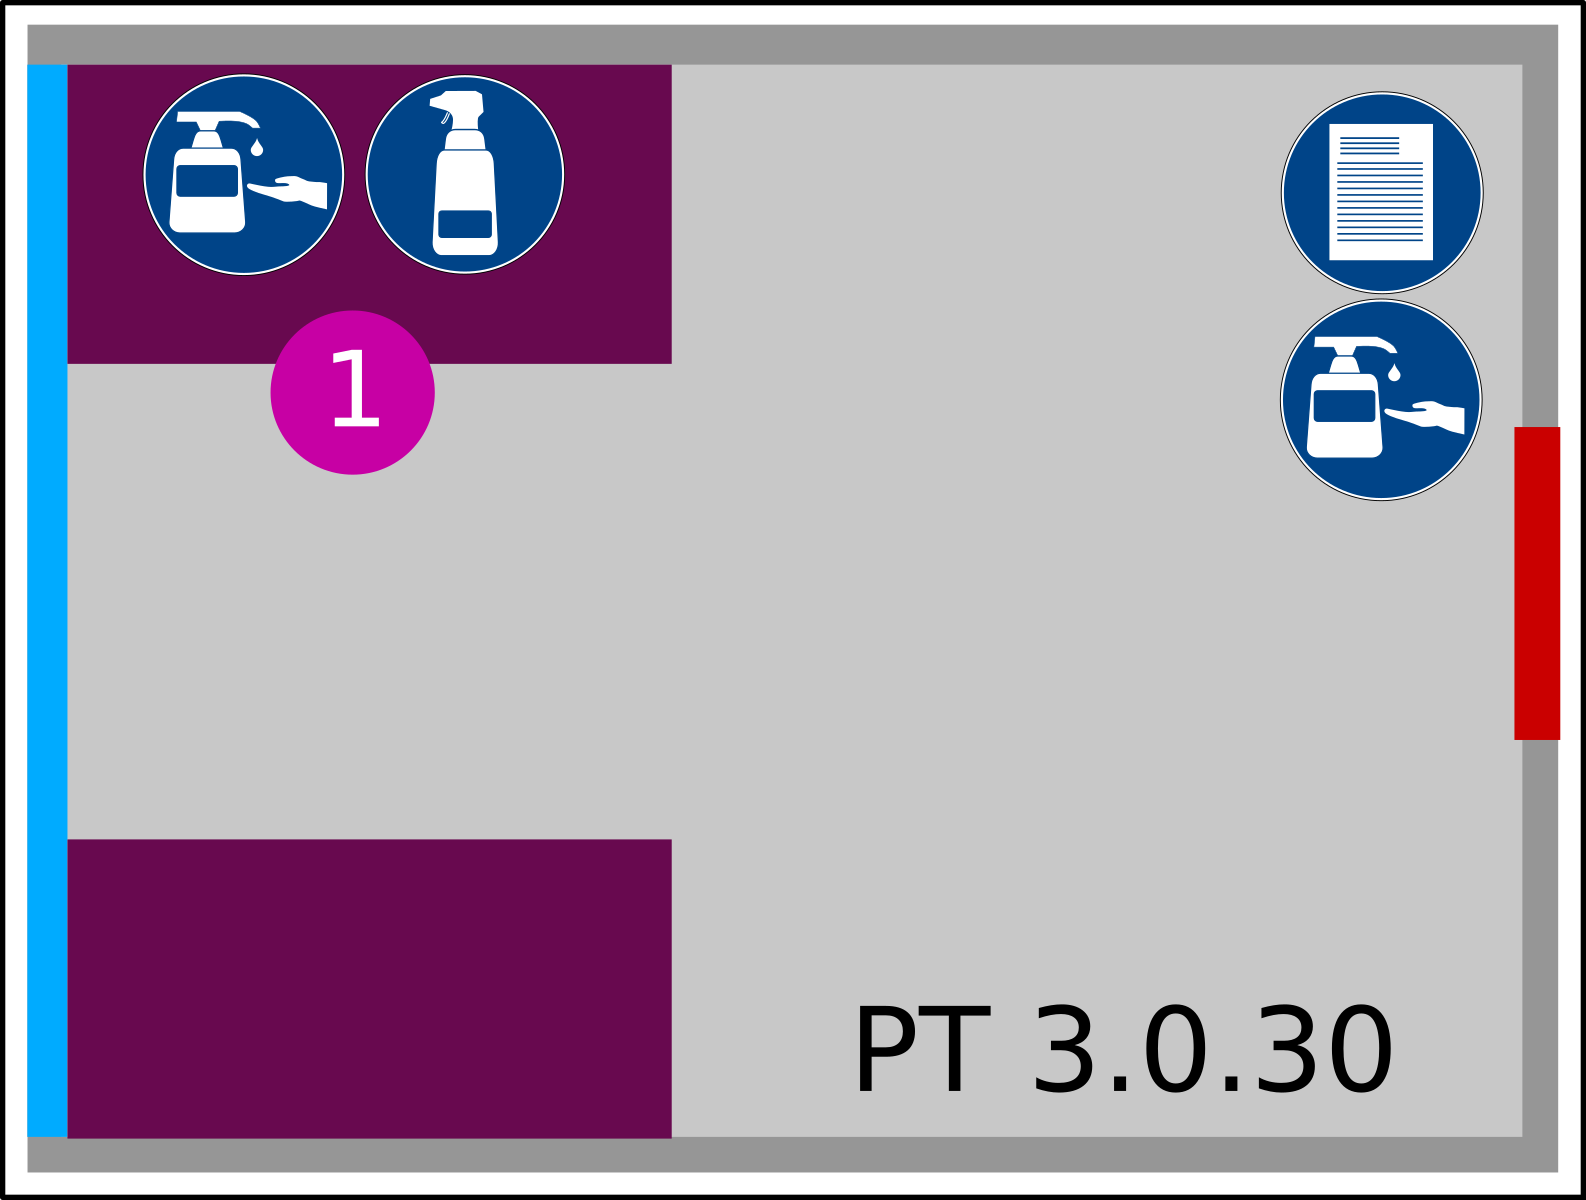
\includegraphics[width=0.7\textwidth]{pt_3_0_30_konzept}
    \caption{Raumplan PT 3.0.30}
\end{figure}

\subsection{Eyetracking-Classroom}\label{subsec:labore_eyetracking}

\labinfo{(prallele) Eye-Tracking-Experimente}{4 (Zusätzliche Arbeitsplätze im Nebenraum vorhanden)}{Alexander Bazo (UR), Forian Hauser (OTH)}

\noindent
Im Classroom stehen 11 Hochleistungs-Eyetracker an separaten Arbeitsplätzen bereit.
Diese sind in Form eines CIP-Pool-Layouts angeordnet (vier Sitzreihen mit je 2 bis 3 Arbeitsplätzen).
Bei entsprechender Einhaltung der Abstandsregel beim Eintritt in den Raum kann pro Sitzreihe ein Arbeitsplatz genutzt werden.
Im Idealfall können so auch Experimente durchgeführt werden, die eine gleichzeitige Nutzung des Labors durch mehrere Probanden erfordern.
Durch den angeschlossenen Nebenraum können separate Ein- und Ausgänge für den Laborraum geschaffen werden.
Nach der Verwendung der Arbeitsplätze werden diese desinfiziert, insbesondere die Tastaturen, Monitore und Oberflächen der Eye-Tracker.
Durch die Reduzierung der verwendeten Eye-Tracker pro Sitzreihe können die verwendeten Geräte zwischen einzelnen Studien alterniert werden.

\medskip

\noindent
\textbf{Jedwede Verwendung des Classrooms wird zwischen den Betreibern (OTH Regensburg, Prof. Mottok und Uni Regensburg, Prof. Wolff und Prof. Gruber) abgestimmt.}

\subsection{TechBase VR4: Labor}\label{subsec:labore_vr4_labor}

\labinfo{Entwicklungsarbeit, Arbeit an interaktiven Tischen}{3}{Andreas Schmid, Raphael Wimmer}

\noindent
Das Labor ist der Hauptraum des VR4. Er bietet Platz für zu drei Personen, die gleichzeitig darin arbeiten können, ohne den Mindestabstand zu unterschreiten. In diesem Raum wird vorwiegend im Rahmen von Abschlussarbeiten an Projekten mit interaktiven Tischen und Projektionen gearbeitet, die auf die bestehende Laborinfrastruktur (beispielsweise Traversen) angewiesen sind.
Es werden persönliche Arbeitsbereiche für jede/n Labornutzer:in eingerichtet, welche nur von diesen benutzt werden.
Diese Arbeitsbereiche werden so platziert, dass noch genügend Abstand zum Durchgang Richtung Studio und Werkstatt besteht.

\subsection{TechBase VR4: Studio}\label{subsec:labore_vr4_stuio}

\labinfo{Entwicklung von VR-Anwendungen, Motion Capturing, Nutzerstudien}{2}{Martin Kocur, Martin Brockelmann}

\noindent
Das VR4-Studio wird genutzt, um Prototypen zu entwickeln und Nutzerstudien im Bereich Virtual Reality (VR) durchzuführen.
Grundsätzlich ist die Nutzung des Studios für die Entwicklung sowie Nutzerstudien gestattet, jedoch dürfen sich nur maximal zwei Personen gleichzeitig im Studio befinden.
Mit Hilfe von Bodenmarkierungen werden entsprechende Bereiche gekennzeichnet, die die Arbeit im Studio und den Ablauf von Studien koordinieren sollen.
VR erfordert das Tragen von Head-Mounted Displays (HMDs), die nach dem Tragen unbedingt gründlich desinfiziert \sout{und für 72 h in einer verschließbaren Box in Quarantäne gesetzt} werden müssen (vgl. Abschnitt \ref{subsec:nutzerstudien_hmd}).
Motion Capturing-Anzüge werden direkt nach dem Tragen zur Reinigung gebracht (vgl. Abschnitt \ref{subsec:nutzerstudien_mocap}).
Werden HMDs von einer Person über einen längeren Zeitraum nur für die Entwicklung von Prototypen verwendet, können diese personalisiert werden, sodass das entsprechende Gerät während dieses Zeitraums ausschließlich von einer Person verwendet wird.
Um die HMDs zu personalisieren, werden eindeutig sichtbare Aufkleber verwendet und eine Liste eingetragen.
Nach jeder Nutzung der im Studio genutzten Geräte und Arbeitsflächen werden diese desinfiziert.
\sout{Da der Raum über keine Fenster verfügt, muss der Raum bei einem Wechsel der Besetzung für mindestens drei Stunden leer stehen. Dies gilt auch für wechselnde Proband:innen bei Nutzerstudien.}
Das VR4-Studio wird über eine RLT-Anlage belüftet.
Zusätzlich soll eine dauerhafte Lüftung über die Türen zum Hauptraum erfolgen, solange sich niemand darin befindet.

\subsection{TechBase VR4: Werkstatt}\label{subsec:labore_vr4_werkstatt}

\labinfo{Bau von Prototypen, Elektronikarbeitsplätze}{1}{Andreas Schmid, Raphael Wimmer}

\noindent
Die Werkstatt wird genutzt um Prototypen für neuartige Geräte zu bauen.
Dazu stehen Werkzeuge wie Lötstationen, Netzteile, ein Oszilloskop, Sägen und Akkuschrauber zur Verfügung.
Grundsätzlich ist die Nutzung der Werkstatt gestattet, jedoch kann aufgrund der geringen Größe nur eine Person gleichzeitig darin arbeiten.
Da Werkzeug und Bauteile teilweise schwer zu desinfizieren sind, wird auf große zeitliche Abstände bei der konsekutiven Nutzung geachtet, um das Risiko von Schmierinfektionen zu verringern.
Die Tür vom Labor zur Werkstatt darf nur zum Betreten und Verlassen des Raums geöffnet werden.


\clearpage

\appendix

\section{Hinweisschilder und Aushänge}

\subsection{Hinweisschild: Hygienehinweise}

\frame{\includegraphics[width=\textwidth]{{hygienehinweis}}}

\subsection{Hinweisschild: Symptome}

\frame{\includegraphics[width=\textwidth]{{symptome}}}

\subsection{Hinweisschild: VR-Nutzerstudien}

\frame{\includegraphics[width=\textwidth]{{hmd}}}

\subsection{Hinweisschild: Check-in}

\frame{\includegraphics[width=\textwidth]{{checkin}}}

\subsection{Hinweisschild: Check-out}

\frame{\includegraphics[width=\textwidth]{{checkout}}}

\subsection{Hygieneprotokoll}

\frame{\includegraphics[width=1.4\textwidth, angle=270]{{hygieneprotokoll}}}

\section{Raumpläne}


\begin{center}
    \sffamily
    \frame{
    \begin{tabular}{ m{1.1cm} m{3cm} }
        \multicolumn{2}{l}{\textbf{Legende}} \\
        \vspace{2mm}
        
\includegraphics[width=1cm]{arbeitsplatz} & Arbeitsplatz \\
        
\includegraphics[width=1cm]{tisch} & Tisch \\
        
\includegraphics[width=1cm]{durchgang} & Tür \\
        
\includegraphics[width=1cm]{fenster} & Fenster \\
        
\includegraphics[width=1cm]{trennwand} & Trennwand \\
    \end{tabular}
    \quad
    \begin{tabular}{ m{1.1cm} m{5cm} }
        \vspace{2mm}
        \includegraphics[width=1cm]{flächendesinfektion} & Flächendesinfektionsmittel \\
        
\includegraphics[width=1cm]{handdesinfektion} & Händedesinfektionsmittel \\
        
\includegraphics[width=1cm]{waschbecken} & Waschbecken \\
        
\includegraphics[width=1cm]{hinweisschilder} & Hinweisschilder \\
    \end{tabular}
    }
\end{center}

\subsection{Future Interaction Lab}

\frame{\includegraphics[width=\textwidth]{{fil_konzept}}}

%\begin{center}
%    \frame{\includegraphics[width=1.45\textwidth, angle=270]{{fil_konzept}}}
%\end{center}

\subsection{Eyetracking-Classroom}

\frame{\includegraphics[width=\textwidth]{{eyetracking-classroom_konzept}}}

\subsection{TechBase: VR4}

\frame{\includegraphics[width=\textwidth]{{vr4_konzept}}}

\end{document}
